\documentclass[12pt,a4paper]{article}
\usepackage[spanish]{babel}
\usepackage[utf8]{inputenc}
\usepackage[T1]{fontenc}
\usepackage{graphicx}
\usepackage{longtable}
\usepackage{geometry}
\geometry{margin=2.5cm}
\title{Reporte Academico: Robot Minisumo}
\author{Proyecto basado en Arduino Nano}
\date{2026-06-05}
\begin{document}
\maketitle
\tableofcontents
\section{Introduccion}
El Robot Minisumo usa Arduino Nano, Shield de expansion, HC-SR04, tres TCRT5000, dos SG90 y buzzer KY-012.
\section{Objetivo General}
Actualizar y consolidar el proyecto para que hardware, firmware, KiCad y documentacion coincidan.
\section{Materiales}
\begin{longtable}{lll}
Componente & Cantidad & Funcion \\
Arduino Nano & 1 & Control \\
Shield Nano & 1 & Conexion \\
HC-SR04 & 1 & Oponente \\
TCRT5000 & 3 & Borde \\
SG90 & 2 & Traccion si son continuos \\
KY-012 & 1 & Buzzer \\
\end{longtable}
\section{Pinout}
\begin{longtable}{lll}
Componente & Senal & Pin \\
TCRT5000 Left & DO & D2 \\
TCRT5000 Right & DO & D3 \\
TCRT5000 Back & DO & D6 \\
HC-SR04 & Trig & D4 \\
HC-SR04 & Echo & D5 \\
KY-012 & Signal & D7 \\
SG90 Left & Signal & D9 \\
SG90 Right & Signal & D10 \\
\end{longtable}
D0/D1 quedan reservados para RX/TX Serial.
\section{Diagrama}
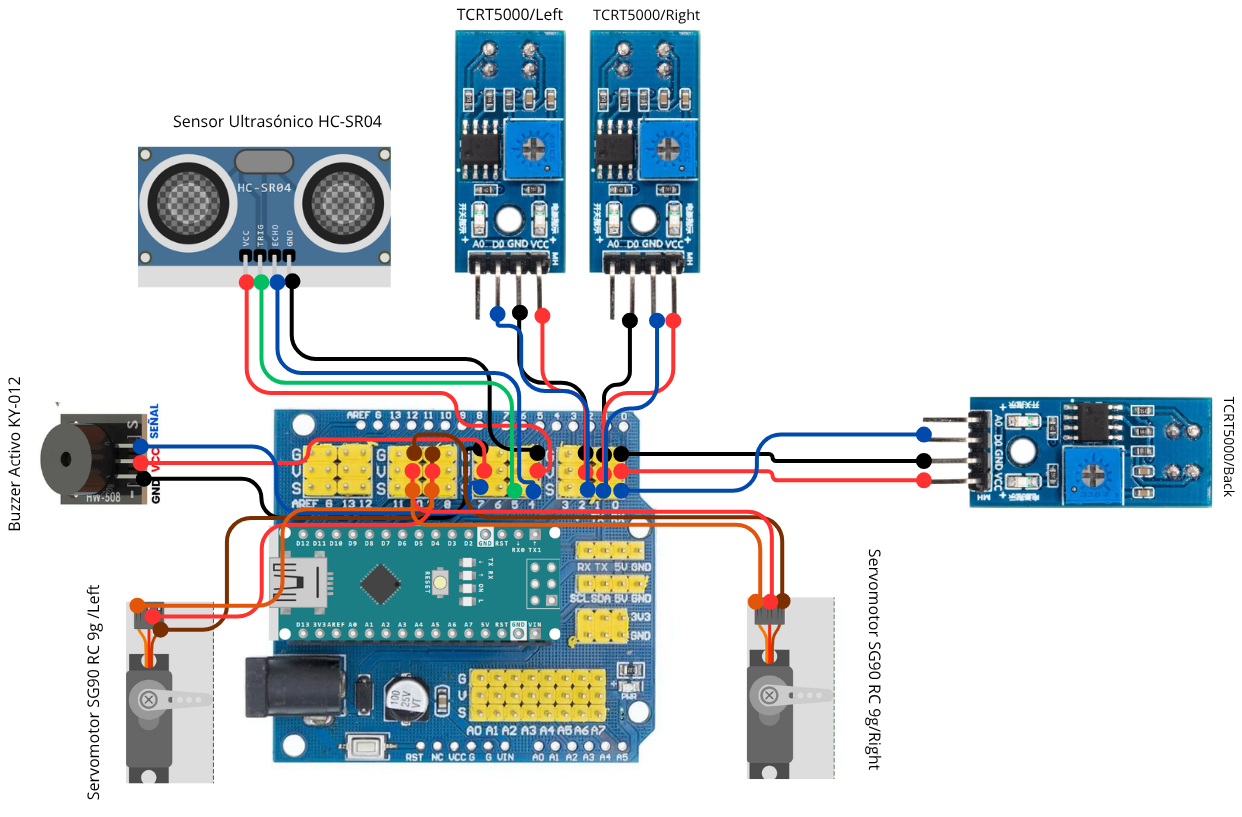
\includegraphics[width=0.95\textwidth]{assets/diagrama_conexiones.png}
\section{Firmware}
El firmware se encuentra en \texttt{firmware/robot\_minisumo\_final/robot\_minisumo\_final.ino}.
\section{Pendientes Criticos}
Confirmar si los SG90 son de rotacion continua y validar alimentacion de servos.
\section{Conclusiones}
El proyecto queda consolidado con pinout seguro y listo para validacion fisica y GitHub.
\end{document}
